\documentclass[polish,polish,a4paper]{article}
\usepackage[utf8]{inputenc}
\usepackage[T1]{fontenc}
\usepackage[polish]{babel}
\usepackage{anysize}
\usepackage{siunitx}
\usepackage{graphicx}
\usepackage{listings}
\usepackage{xcolor} % do komentarzy

\marginsize{2.5cm}{2.5cm}{2cm}{2cm}

\title{Symulator tomografu komputerowego}
\author{Przemysław Ambroży, Błażej Celmer}

\begin{document} 
	\maketitle
	
 	\section{Model}
		\begin{center}
			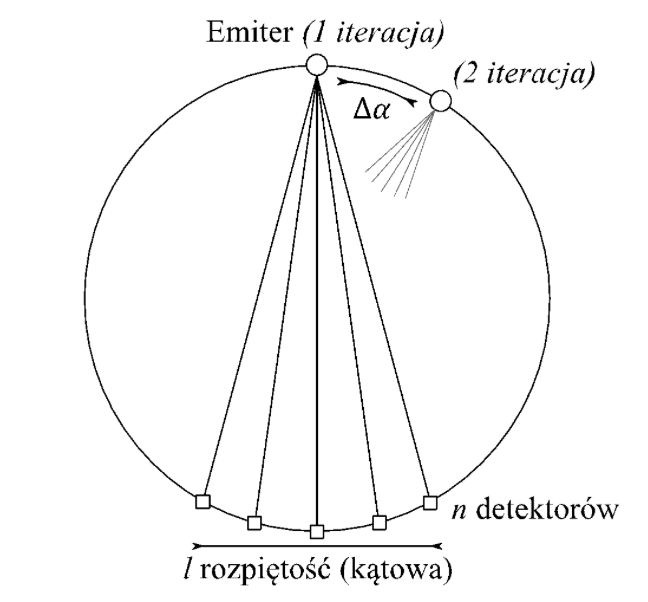
\includegraphics[scale=0.7]{img/model.png} \\
			\small{rys. 1. model stożkowy}
		\end{center}
		Zastosowany został model stożkowy (rys. 1.).
		 Zakłada on wykorzystanie jednego emitera,
		  który współpracuje ze wszystkimi detektorami, tworząc wspomniany stożek 
		  (W przeciwieństwie do modelu równoległego, gdzie każdy detektor posiada własny emiter).
		 {\color{red}  coś bym tu jeszcze dopisał }
		
	\section{Program}
		\subsection{Środowisko}
			Do zasymulowania tomografu skorzystaliśmy z języka Python w środowisku Jupyter Notebook,
			 co pozwoliło niskim kosztem uzyskać interfejs użytkownika.
			 Skorzystaliśmy również z bibliotek, które oferowały dodatkowe funkcjonalności, m.in.:
			
			\begin{description}
				\item[numpy] funkcje i stałe matematyczne
				\item[matplotlib] wyświetlanie grafik
				\item[ipywidgets] interfejs użytkownika
				\item[pydicom] odczyt i zapis plików DICOM
			\end{description}
			
			\subsection{Opis działania}
				\subsubsection{Sinogram}
				
				Sinogram, jest to tablica danych, 
				gdzie każdy wiersz to jedna iteracja (pozycja emitera), 
				a każda kolumna oznacza jeden detektor.
				Aby otrzymać sinogram, należy wykonać n iteracji, 
				w których emiter wraz z~detektorami będzie się stopniowo przesuwał po okręgu, 
				aż obrócimy cały układ o 180 stopni. 
				Podczas każdej iteracji wyznaczamy współrzędne punktów, w których znajduje się emiter oraz detektory.
				
				{\color{red} Opis wyznaczana współrzędnych}
				
				Aby pobrać dane z obiektu znajdującego się między emiterem a detektorami (w naszym przypadku z obrazka), wykorzystujemy algorytm \textbf{Bresenhama}. Służy on do wyznaczenia pikseli znajdujących się między dwoma punktami. Przechodzi iteracyjnie przez wszystkie wartości na jednej osi (np. OX, jeśli obrazek jest szerszy niż wyższy). W każdym kroku decyduje, czy wykonać tylko ruch wzdłuż jednej osi (poziomo/pionowo), czy obu (na ukos).
				
				\begin{figure}[!h]
					\centering
					\begin{minipage}{0.4\linewidth}
						\begin{lstlisting}[language=Python, frame=single]
for i in range(x1, x2):
    points.append((i, j))
    if e > 0:
        j += m
        e += 2 * (dy - dx)
    else:
        e += 2 * dy
						\end{lstlisting}
						\caption{Fragment kodu algorytmu}
					\end{minipage}
					\hfill
					\begin{minipage}{0.45\linewidth}
						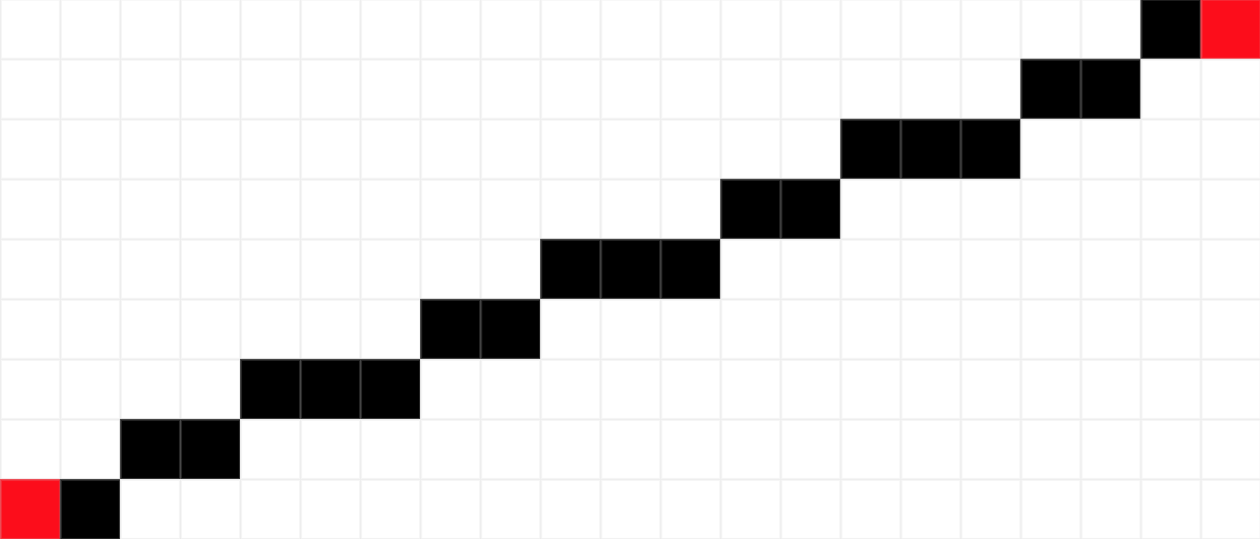
\includegraphics[width=\textwidth]{img/bresenham.png}
						\caption{Przykład działania -- znajdowanie pikseli między dwoma czerwonymi}
					\end{minipage}
				\end{figure}
				
				Znając wszystkie piksele leżące między emiterem, a detektorem, 
				sumujemy ich jasność i zapisujemy w odpowiednim miejscu sinogramu.
				Na koniec normalizujemy wszystkie dane, tak aby wartości były z~przedziału od~0~do~1. W tym celu znajdujemy największą wartość (najjaśniejszy piksel) i dzielimy przez nią pozostałe.
				
				\subsubsection{Obraz wynikowy}
				Sinogram nie jest zrozumiały dla człowieka, 
				dlatego należy go przekształcić.
				Zaczynamy od czarnego obrazu i znów przejdziemy przez n iteracji.
				Każdej iteracji przypisana będzie pozycja emitera wraz z~detektorami 
				(będą to te same pozycje, co podczas generowania sinogramu).
				Wyznaczamy linie przechodzące przez obraz między emiterem i detektorami (algorytm Bresenhama).
				Każdy piksel, przez który przechodzi linia będzie rozjaśniony o wartość odczytaną z sinogramu 
				(dla danego detektora w danej iteracji). 
				Nałożenie wszystkich linii na obrazie stworzy obraz wynikowy.
				{\color{red} to samo co wyżej, no i myślę jeszcze o jakiś obrazkach}
			\subsection{Standard DICOM}
\end{document}
